\documentclass{standalone}
\begin{document}
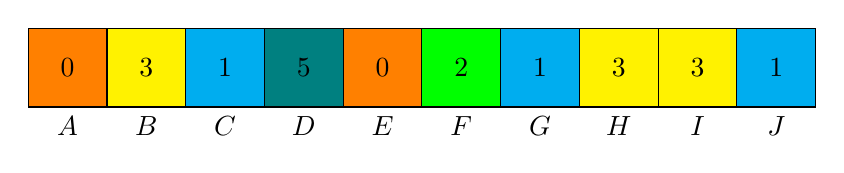
\begin{tikzpicture}


\fill[orange] (0, 0) rectangle (1, 1);
\fill[yellow] (1, 0) rectangle (2, 1);
\fill[cyan] (2, 0) rectangle (3, 1);
\fill[teal] (3, 0) rectangle (4, 1);
\fill[orange] (4, 0) rectangle (5, 1);

\fill[green] (5, 0) rectangle (6, 1);
\fill[cyan] (6, 0) rectangle (7, 1);
\fill[yellow] (7, 0) rectangle (8, 1);
\fill[yellow] (8, 0) rectangle (9, 1);
\fill[cyan] (9, 0) rectangle (10, 1);

\draw (0, 0) -- (10, 0);
\draw (0, 1) -- (10, 1);
\foreach \i in {0,...,10}
{
    \draw (\i,0) -- (\i, 1);
}

\draw ( 0.5, 0) node[below]{$A$};
\draw ( 1.5, 0) node[below]{$B$};
\draw ( 2.5, 0) node[below]{$C$};
\draw ( 3.5, 0) node[below]{$D$};
\draw ( 4.5, 0) node[below]{$E$};

\draw ( 5.5, 0) node[below]{$F$};
\draw ( 6.5, 0) node[below]{$G$};
\draw ( 7.5, 0) node[below]{$H$};
\draw ( 8.5, 0) node[below]{$I$};
\draw ( 9.5, 0) node[below]{$J$};

% grid indices
\draw ( 0.5, .5) node[]{$0$};
\draw ( 1.5, .5) node[]{$3$};
\draw ( 2.5, .5) node[]{$1$};
\draw ( 3.5, .5) node[]{$5$};
\draw ( 4.5, .5) node[]{$0$};

\draw ( 5.5, .5) node[]{$2$};
\draw ( 6.5, .5) node[]{$1$};
\draw ( 7.5, .5) node[]{$3$};
\draw ( 8.5, .5) node[]{$3$};
\draw ( 9.5, .5) node[]{$1$};


\end{tikzpicture}
\end{document}
